\documentclass[12pt]{article}
\usepackage{amsmath}
\usepackage{graphicx}
\usepackage{hyperref}
\usepackage{listings}
\usepackage{color}
\usepackage{pythonhighlight}

\title{Operating System Course Report - First Half of the Semester}
\author{B class}
\date{\today}

\begin{document}

\maketitle
\newpage

\tableofcontents
\newpage

\section{Introduction}
This report summarizes the topics covered during the first half of the Operating System course. It includes theoretical concepts, practical implementations, and assignments. The course focuses on the fundamentals of operating systems, including system architecture, process management, CPU scheduling, and deadlock handling.

\section{Course Overview}
\subsection{Objectives}
The main objectives of this course are:
\begin{itemize}
    \item To understand the basic components and architecture of a computer system.
    \item To learn process management, scheduling, and inter-process communication.
    \item To explore file systems, input/output management, and virtualization.
    \item To study the prevention and handling of deadlocks in operating systems.
\end{itemize}

\subsection{Course Structure}
The course is divided into two halves. This report focuses on the first half, which covers:
\begin{itemize}
    \item Basic Concepts and Components of Computer Systems
    \item System Performance and Metrics
    \item System Architecture of Computer Systems
    \item Process Description and Control
    \item Scheduling Algorithms
    \item Process Creation and Termination
    \item Introduction to Threads
    \item File Systems
    \item Input and Output Management
    \item Deadlock Introduction and Prevention
    \item User Interface Management
    \item Virtualization in Operating Systems
\end{itemize}

\section{Topics Covered}

\subsection{Basic Concepts and Components of Computer Systems}
This section explains the fundamental components that make up a computer system, including the CPU, memory, storage, and input/output devices.

\subsection{System Performance and Metrics}
This section introduces various system performance metrics used to measure the efficiency of a computer system, including throughput, response time, and utilization.

\subsection{System Architecture of Computer Systems}
\subsubsection{Interaksi antara Hardware dengan Sistem Operasi}
Sistem Operasi (OS) berperan sebagai penghubung antara perangkat keras ( \textit{hardware}) dan perangkat lunak (\textit{software}) yang dijalankan oleh pengguna. Sistem operasi mengelola dan mengatur semua komponen perangkat keras agar dapat berfungsi secara efisien. Ada beberapa cara interaksi antara \textit{hardware} dengan sistem operasi:
\begin{itemize}
    \item Penglolaan Sumber Daya \textit{Hardware}: Sistem operasi mengatur penggunaan perangkat keras seperti CPU, memori, dan perangkat \textit{input/output} (I/O) berdasarkan kebutuhan perangkat lunak dan pengguna. Proses ini mencakup pengelolaan memori, penjadwalan tugas, dan manajemen textit{file}. Dengan cara ini, OS memastikan bahwa sumber daya tersebut digunakan secara optimal untuk berbagai proses yang berjalan di komputer.
    \item Kontrol Arus Data: Sistem operasi mengendalikan aliran data antara perangkat keras dan perangkat lunak. Ketika perangkat keras mengirimkan data, OS memastikan bahwa data tersebut diterima dan diproses oleh perangkat lunak dengan benar. Sebaliknya, OS juga memastikan bahwa instruksi dari perangkat lunak dapat dikirim ke perangkat keras tanpa masalah.
    \item Driver: Sistem operasi menggunakan \textit{driver} untuk berkomunikasi dengan perangkat keras. \textit{Driver} adalah perangkat lunak spesifik yang mengendalikan perangkat keras, seperti \textit{printer}, kartu jaringan, atau perangkat penyimpanan. Tanpa \textit{driver} yang tepat, perangkat keras tidak dapat dikenali atau digunakan oleh OS.
    \item \textit{Interrupt Handling}: Ketika perangkat keras membutuhkan perhatian segera, seperti saat ada \textit{input} dari keyboard atau \textit{mouse}, perangkat tersebut mengirimkan \textit{interrupt} ke CPU. Sistem operasi akan menghentikan sementara proses yang sedang berjalan untuk menangani \textit{interrupt} tersebut, kemudian mengembalikan kontrol ke proses sebelumnya setelah \textit{interrupt} selesai ditangani.
    \item Manajemen Akses Pengguna: OS mengatur dan mengontrol akses pengguna terhadap perangkat keras melalui pengaturan hak akses dan izin. Sistem operasi memastikan bahwa setiap pengguna hanya dapat mengakses sumber daya yang relevan dengan tugas atau peran mereka, menjaga keamanan dan integritas sistem.
    \item \textit{Direct Memory Access} (DMA): OS menggunakan DMA untuk memungkinkan perangkat keras tertentu, seperti perangkat penyimpanan, berinteraksi langsung dengan memori tanpa memerlukan campur tangan CPU. Ini mempercepat proses transfer data dan mengurangi beban kerja CPU.
    \item \textit{System Calls}: \textit{System calls} adalah antarmuka yang digunakan oleh perangkat lunak untuk meminta layanan dari OS, termasuk layanan yang terkait dengan perangkat keras. Dengan \textit{system calls}, perangkat lunak dapat berinteraksi dengan perangkat keras melalui OS, tanpa harus langsung mengendalikan perangkat keras tersebut. Hal ini memastikan keamanan dan kestabilan sistem secara keseluruhan.
\end{itemize}

\subsection{Process Description and Control}
Processes are a central concept in operating systems. This section covers:
\begin{itemize}
    \item Process states and state transitions
    \item Process control block (PCB)
    \item Context switching
\end{itemize}

\subsection{Scheduling Algorithms}
This section covers:
\begin{itemize}
    \item First-Come, First-Served (FCFS)
    \item Shortest Job Next (SJN)
    \item Round Robin (RR)
\end{itemize}
It explains how these algorithms are used to allocate CPU time to processes.

\subsection{Process Creation and Termination}
Details how processes are created and terminated by the operating system, including:
\begin{itemize}
    \item Process spawning
    \item Process termination conditions
\end{itemize}

\subsection{Introduction to Threads}
This section introduces the concept of threads and their relation to processes, covering:
\begin{itemize}
    \item Single-threaded vs. multi-threaded processes
    \item Benefits of multithreading
\end{itemize}

\begin{figure}[h]
    \centering
    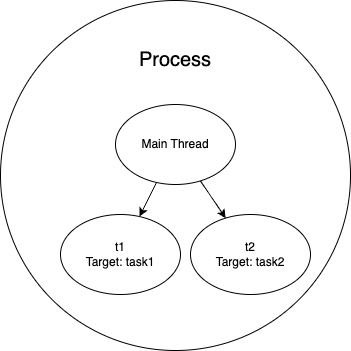
\includegraphics[width=0.5\textwidth]{/Users/khawaritzmi/Unhas/os_report_mid2024/b_class/asset/example.png}  % Sesuaikan nama file dan ukurannya
    \caption{Ini adalah gambar contoh dari multithreading.}
    \label{fig:contoh_gambar}
\end{figure}

Seperti yang terlihat pada Gambar \ref{fig:contoh_gambar}, inilah cara menambahkan gambar dengan keterangan.

\subsection{File Systems}
File systems provide a way for the operating system to store, retrieve, and manage data. This section explains:
\begin{itemize}
    \item File system structure
    \item File access methods
    \item Directory management
\end{itemize}

\subsection{Input and Output Management}
Input and output management is key for handling the interaction between the system and external devices. This section includes:
\begin{itemize}
    \item Device drivers
    \item I/O scheduling
\end{itemize}

\subsection{Deadlock Introduction and Prevention}
Explores the concept of deadlocks and methods for preventing them:
\begin{itemize}
    \item Deadlock conditions
    \item Deadlock prevention techThis assignment involved designing a multithreading scenario to solve a computationally intensive problem. Students then applied **Amdahl's Law** to calculate the theoretical speedup of the program as the number of threads increased.
niques
\end{itemize}

\subsection{User Interface Management}
This section discusses the role of the operating system in managing the user interface. Topics covered include:
\begin{itemize}
    \item Graphical User Interface (GUI)
    \item Command-Line Interface (CLI)
    \item Interaction between the user and the operating system
\end{itemize}

\subsection{Virtualization in Operating Systems}
Virtualization allows multiple operating systems to run concurrently on a single physical machine. This section explores:
\begin{itemize}
    \item Concept of virtualization
    \item Hypervisors and their types
    \item Benefits of virtualization in modern computing
\end{itemize}

\section{Assignments and Practical Work}
\subsection{Assignment 1: Process Scheduling}
Students were tasked with implementing various process scheduling algorithms (e.g., FCFS, SJN, and RR) and comparing their performance under different conditions.
\subsubsection{Group 1}
\begin{python}
    class Process:
    def __init__(self, pid, arrival_time, burst_time):
        self.pid = pid
        self.arrival_time = arrival_time
        self.burst_time = burst_time
        self.completion_time = 0
        self.turnaround_time = 0
        self.waiting_time = 0
\end{python}

\begin{table}[htbp] % Optional: For floating position
    \centering
    \begin{tabular}{|c|c|c|} % Defines number of columns and alignment (c = center, l = left, r = right). '|' creates vertical lines.
    \hline
    Header 1 & Header 2 & Header 3 \\ % Column headers
    \hline
    Row 1, Column 1 & Row 1, Column 2 & Row 1, Column 3 \\ % First row of data
    \hline
    Row 2, Column 1 & Row 2, Column 2 & Row 2, Column 3 \\ % Second row of data
    \hline
    \end{tabular}
    \caption{Your table caption} % Optional: For adding a caption
    \label{tab:your_label} % Optional: For cross-referencing the table
\end{table}

\subsection{Assignment 2: Deadlock Handling}
In this assignment, students were asked to simulate different deadlock scenarios and explore various prevention methods.

\subsection{Assignment 3: Multithreading and Amdahl's Law}
\subsubsection{Group 3}
Soal 1 :
Anda diminta untuk membuat program Python yang menggunakan multithreading untuk menghitung jumlah bilangan prima dalam rentang angka dari 1 hingga 
N.Program harus membagi rentang ini menjadi beberapa bagian dan memprosesnya secara paralel untuk meningkatkan kinerja. Implementasikan program yang menghitung jumlah bilangan prima dalam rentang 1 hingga 
N menggunakan multithreading. Hitung dan tampilkan waktu eksekusi program untuk jumlah thread yang berbeda (misalnya 1, 2, 4, 8). Catat hasil jumlah bilangan prima dan waktu eksekusi yang didapat.

jawaban:
\begin{python}
    import threading
    import time
    import math

    def is_prime(n):
        if n <= 1:
            return  False
        for i in range(2, int(math.sqrt(n)) + 1)
            if n % 1 == 0:
                return False
        return True

        def count_primes_in_range(start, end, results, index):
            prime_count = 0
        for num in range(start, end):
            if is_prime(num):
                prime_count += 1
        results[index] = prime_count

        def multithreaded_prime_count(n, num_threads):
            threads = []
            results = [0] * num_threads
            range_size = n // num_threads

            for i in range(num_threads):
                start = i * range_size
                end = (i + 1) * range_size 
                if i != num_threads - 1 else n
                t = threading.Thread
                (target=count_primes_in_range, 
                args=(start, end, results, i))
                threads.append(t)

            start_time = time.time()

            for t in threads:
                t.start()

            for t in threads:
                t.join()

            end_time = time.time()

            total primes = sum(results)
            execution_time = end_time - start_time

            return total_primes, execution_time

    if __name__ == "__main__":
        N = 100000
        num_threads_list = [1, 2, 4, 8]

        for num_threads in num_threads_list:
        primes, exec_time = multithreaded_prime_count(N, num_threads)
        print(f"Jumlah thread: {num_threads}, Jumlah bilangan prima: {primes}, 
        Waktu eksekusi: {exec_time:.4f} detik")
    \end{python}

Contoh Output Soal 1:
\begin{itemize}
    \item Jumlah thread: 1, Jumlah bilangan prima: 9592, Waktu eksekusi: 3.2435 detik
    \item Jumlah thread: 2, Jumlah bilangan prima: 9592, Waktu eksekusi: 1.6521 detik
    \item Jumlah thread: 4, Jumlah bilangan prima: 9592, Waktu eksekusi: 0.8534 detik
    \item Jumlah thread: 8, Jumlah bilangan prima: 9592, Waktu eksekusi: 0.5321 detik
\end{itemize}

Soal 2:
Setelah menyelesaikan tugas pertama, Anda diminta untuk menghitung speedup teoritis menggunakan Hukum Amdahl berdasarkan program yang telah Anda buat. Anda akan mengasumsikan proporsi 
P dari kode yang dapat diparalelisasi dan menghitung speedup untuk beberapa jumlah thread. Implementasikan fungsi untuk menghitung speedup teoritis menggunakan Hukum Amdahl dan tampilkan speedup teoritis untuk beberapa nilai 
N dan P berdasarkan jumlah thread yang digunakan di Soal 1.
Gunakan hasil dari Soal 1 untuk membandingkan waktu eksekusi aktual dengan speedup teoritis.
Jawaban:
\begin{python}
    def amdahls_law(p, n):
    return 1 / ((1 - p) + (p / n))

if _name_ == "_main_":
    p = 0.95 
    num_threads_list = [1, 2, 4, 8] 

    print("\nMenghitung Speedup Teoritis menggunakan Hukum Amdahl:")
    for num_threads in num_threads_list:
        theoretical_speedup = amdahls_law(p, num_threads)
        print(f"Jumlah thread: {num_threads}, Speedup 
        Teoritis: {theoretical_speedup:.4f}")
\end{python}
Contoh Output Soal 2:
\begin{itemize}
    \item Menghitung Speedup Teoritis menggunakan Hukum Amdahl:
    \item Jumlah thread: 1, Speedup Teoritis: 1.0000
    \item Jumlah thread: 2, Speedup Teoritis: 1.9048
    \item Jumlah thread: 4, Speedup Teoritis: 3.6923
    \item Jumlah thread: 8, Speedup Teoritis: 6.0000
\end{itemize}

\subsection{Assignment 4: Simple Command-Line Interface (CLI) for User Interface Management}
Students were tasked with creating a simple **CLI** for user interface management. The CLI should support basic commands such as file manipulation (creating, listing, and deleting files), process management, and system status reporting.

\subsection{Assignment 5: File System Access}
In this assignment, students implemented file system access routines, including:
\begin{itemize}
    \item File creation and deletion
    \item Reading from and writing to files
    \item Navigating directories and managing file permissions
\end{itemize}

\section{Conclusion}
The first half of the course introduced core operating system concepts, including process management, scheduling, multithreading, and file system access. These topics provided a foundation for more advanced topics to be covered in the second half of the course.

\section{References}
- Tanenbaum, A. S., & Bos, H. (2014). \textit{Modern Operating Systems} (4th ed.). Pearson.
- Stallings, W. (2018). \textit{Computer Organization and Architecture} 
- Telkom University. (n.d.). \textit{Mengenal Sistem Operasi Komputer}. Diambil dari https://www.telkomuniversity.ac.id/mengenal-sistem-operasi
\end{document}